\documentclass[transmag]{IEEEtran}
\usepackage{latexsym}
\usepackage{float}
\usepackage{subcaption}
\usepackage{graphicx}
\usepackage{amsfonts,amssymb,amsmath}
\usepackage{hyperref}
\usepackage{booktabs}
\usepackage[spanish]{babel}
\renewcommand{\spanishtablename}{Tabla}
\def\BibTeX{{\rm B\kern-.05em{\sc i\kern-.025em b}\kern-.08em T\kern-.1667em\lower.7ex\hbox{E}\kern-.125emX}}

\begin{document}

\title{Reporte final de proyecto}

\author{Diego Isla López}


\IEEEtitleabstractindextext{\begin{abstract}Abstract: El problema de reconocimiento de objetos y formas es uno de los más estudiados tanto en aprendizaje automático como en visión computacional. Se hace un experimento con imágenes de Pokémon para verificar el desempeño de modelos tradicionales de clasificación así como de redes neuronales y hacer una comparación entre ellos.\end{abstract}}

\maketitle

\section{Introducción}


El problema de clasificación y reconocimiento de objetos es un problema clásico en Aprendizaje Automático (AA). En este proyecto se busca probar el rendimiento de métodos clásicos de clasificación y redes neuronales en el reconocimiento de diferentes pokemones. Si bien existe un gran número de pokemones distintos, nos enfocaremos en la identificación de un conjunto de pokemones muy similares, los llamados \textit{eevolution}. Los \textit{eevolution} son pokemones que surgen de la evolución de un mismo pokémon, Eevee, por lo que sus formas son muy parecidas (similares a perros o gatos) y con diferencias específicas en color y forma de alguna parte del cuerpo (figura \ref{fig:eevolution}). En particular, se intentará hacer la prueba de desempeño usando la dinámica de \textit{Who's that Pokémon?} presente en la serie animada de Pokémon. La dinámica consiste en que el televidente adivine qué Pokémon se está mostrando a partir de una ``sombra'' donde la figura del pokemon se presenta en un color sólido y la silueta es la única información usada para adivinar (figura \ref{fig:who}). Existen ocho diferentes \textit{eevolution}: Vaporeon, Jolteon, Flareon, Espeon, Glaceon, Umbreon, Sylveon, Leafeon. Las clases serán representadas con los nombres de dichos pokemon.
 
\begin{figure}[H]
	\begin{subfigure}{0.5\textwidth}
		\centering
		
\includegraphics[width=0.8\linewidth]{who1}
		\caption{Pregunta}
	\end{subfigure}
	\begin{subfigure}{0.5\textwidth}
		\centering
		
\includegraphics[width=0.8\linewidth]{who2}
		\caption{Respuesta}
	\end{subfigure}
	\caption{Dinámica de \textit{Who's that Pokémon?}}
	\label{fig:who}
\end{figure}

\begin{figure}
	\centering
	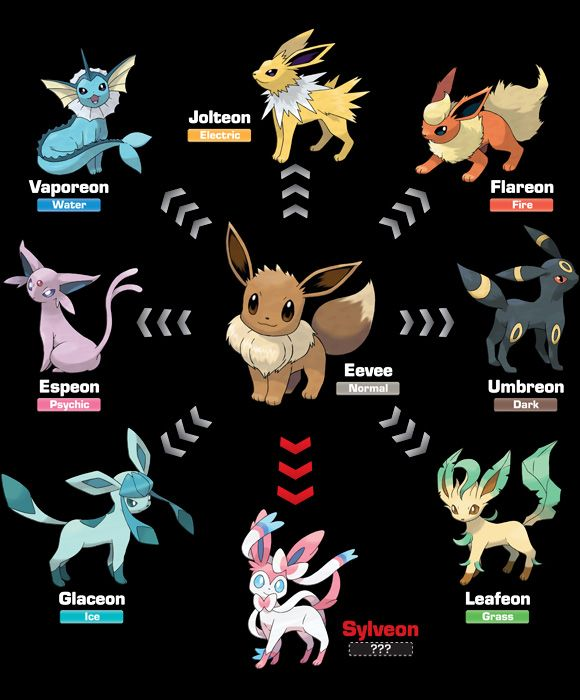
\includegraphics[width=0.8\linewidth]{eevolutions}
	\caption{Los diferentes \textit{eevolution}}
	\label{fig:eevolution}
\end{figure}

De este modo, se utilizará un conjunto de entrenamiento con imágenes a color de cada pokémon y un conjunto de prueba con imágenes en color sólido. Las imágenes a color fueron obtenidas de un conjunto disponible en Kaggle\footnote{Disponible en \url{https://www.kaggle.com/thedagger/pokemon-generation-one}} y mediante \textit{image scraping} usando la búsqueda de Google. Las imágenes sólidas fueron creadas a partir de imágenes transparentes obtenidas de búsquedas en Google, las cuales fueron rellenadas con color negro. 


\section{Estado del arte}

No es difícil imaginar las aplicaciones que puede tener la detección de objetos, desde el área médica hasta seguridad. Dada la popularidad que han ganado las redes neuronales en los últimos años, se han llevado a cabo diversos experimentos además de desarrollo de técnicas nuevas para el problema de clasificación de imágenes. Las redes neuronales convolucionales (CNN) han resultado ser de las más eficientes para abordar este tipo de problemas. Debido a esto, se han propuesto variaciones  a este modelo de redes neuronales. Como se menciona en \cite{zhao2018object}, las ventajas que tienen las CNN sobre los métodos tradicionales de clasificación son:
\begin{itemize}
	\item Exhiben una representación jerárquica de características
	\item Poseen una capacidad expresiva mayor
	\item Ofrecen la oportunidad de optimizar diferentes aspectos de manera simultanea
	\item Hacen posible trasladar ciertos problemas de visión computacional a problemas de transformación de datos a dimensiones mayores.
\end{itemize}             

Recientemente han aparecido modelos como las CNN basadas en regiones (R-CNN), las cuales funcionan determinando un número fijo de regiones de la imagen a evaluar \cite{girshick}; el modelo \textit{You Only Look Once} (YOLO) \cite{redmon2015look}  el cual ha tenido resultados significativos en el reconocimiento de imágenes en video en tiempo real. 

De igual manera, el modelo MobileNets fue propuesto por ingenieros de Google en  \cite{howard2017mobilenets}. Este modelo ha mostrado buen desempeño en problemas varios de visión computacional además de clasificación de imágenes. En los experimentos de este proyecto se utiliza un modelo basado en MobileNets para la implementación con redes neuronales.

Una técnica que ha dado buenos resultados es la de aprendizaje por transferencia (TF) \cite{yosinski2014transferable}, que se refiere a pre-entrenar una red para obtener ciertas características y estás alimentarlas a otra red para poder tener un mejor desempeño de aprendizaje. 
\section{Metodología}

Al ser un problema de clasificación de imágenes es necesario realizar un proceso de extracción de características. Este proceso se refiere a realizar un pre-procesamiento de las imágenes donde se traduce la información de los píxeles y se crea una matriz de características. Esto ayuda a reducir la dimensión y complejidad de las imágenes. Debido a que el conjunto de datos recabado resultó con una cantidad baja de imágenes, se utilizaron técnicas de incremento de datos para tener un conjunto de 2000 imágenes por clase. Para procesar las imágenes aumentadas se utilizaron métodos de ruido, rotaciones e inversiones aleatorias.

\subsection{Métodos tradicionales}

Se hará una comparación entre distintos clasificadores: regresión logística (LR), $ K $-vecinos más cercanos (KNN), bosques aleatorios (RF), descenso por gradiente estocástico (SGD) y máquinas de vectores de soporte (SVM). Para la extracción de características se utilizarán tres métodos:

\begin{itemize}
	\item Momentos de imagen
	\item Texturas Haralick
	\item Histograma de colores
	\item Descriptor KAZE
\end{itemize}

\subsection{Redes neuronales convolucionales}

Se elige un modelo pre-entrenado de Tensorflow\footnote{Disponible en \url{https://tfhub.dev/google/tf2-preview/mobilenet_v2/feature_vector/4}} basado en la arquitectura Mobilenet. Este modelo admite una opción para entrenarse con un conjunto de datos personalizado, por lo que se hacen pruebas con ambas modalidades del modelo.

\section{Experimentación y resultados}

\subsection{Métodos tradicionales}

En la figura \ref{fig:trad} es posible ver que el clasificador RF es el que presenta mejor desempeño entre los modelos tradicionales. En la tabla \ref{tab:res_trad} observamos que la precisión para el modelo RF es de 73.48\% con el conjunto de validación. Sin embargo, al probar el desempeño del modelo con las imágenes de prueba, se observa que el comportamiento no es ideal. Las predicciones apuntan hacia una sola clase para todas las imágenes del conjunto. 

Como se puede ver en la figura \ref{fig:conf_rf} , la matriz de confusión para el modelo muestra la distribución de las predicciones sobre una sola clase.

\begin{figure}[H]
	\centering
	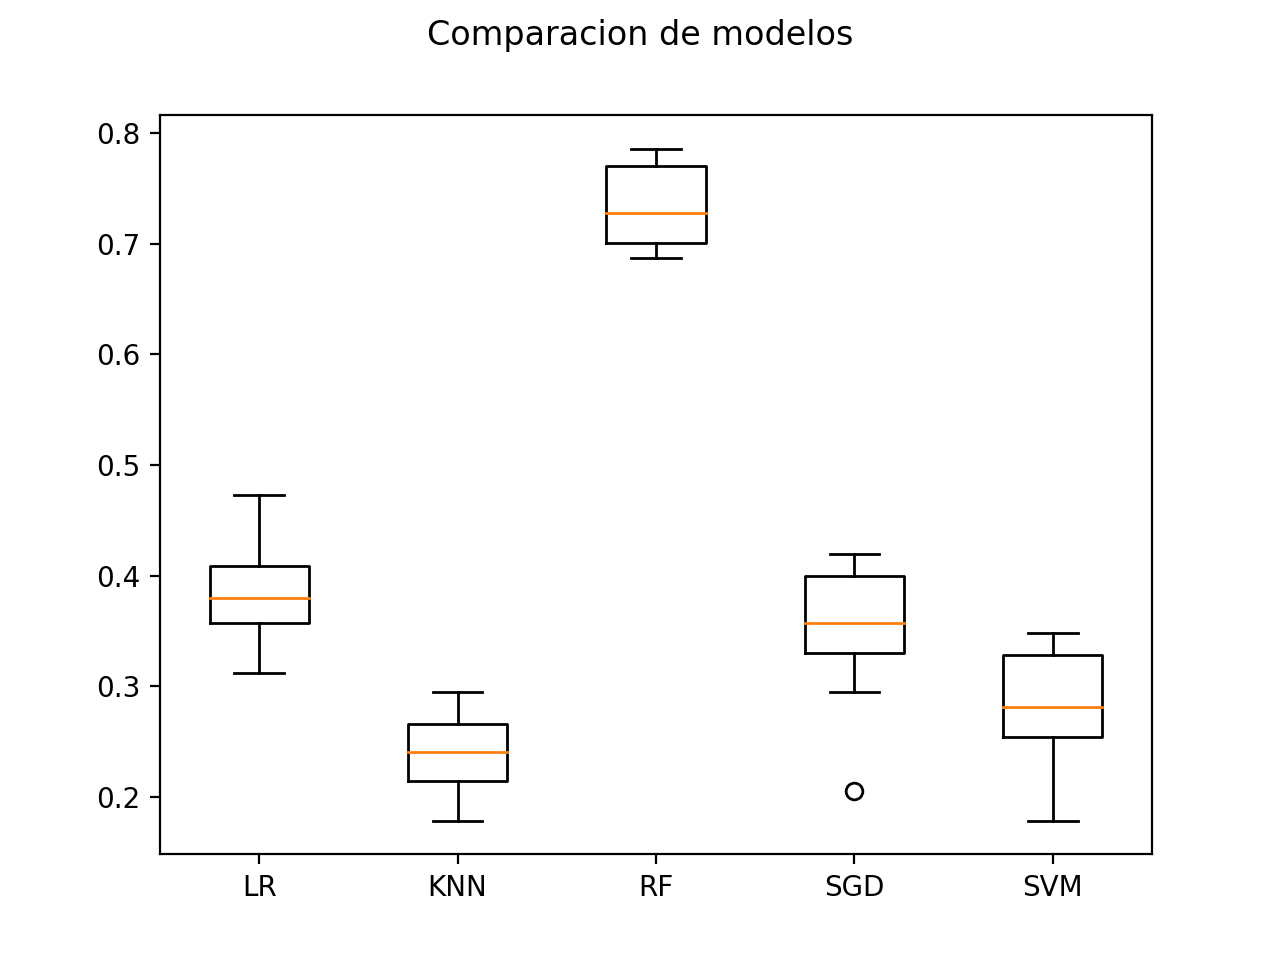
\includegraphics[width=0.8\linewidth]{finaltrad}
	\caption{Desempeño de diferentes clasificadores}
	\label{fig:trad}
\end{figure}


\begin{figure}[H]
\centering
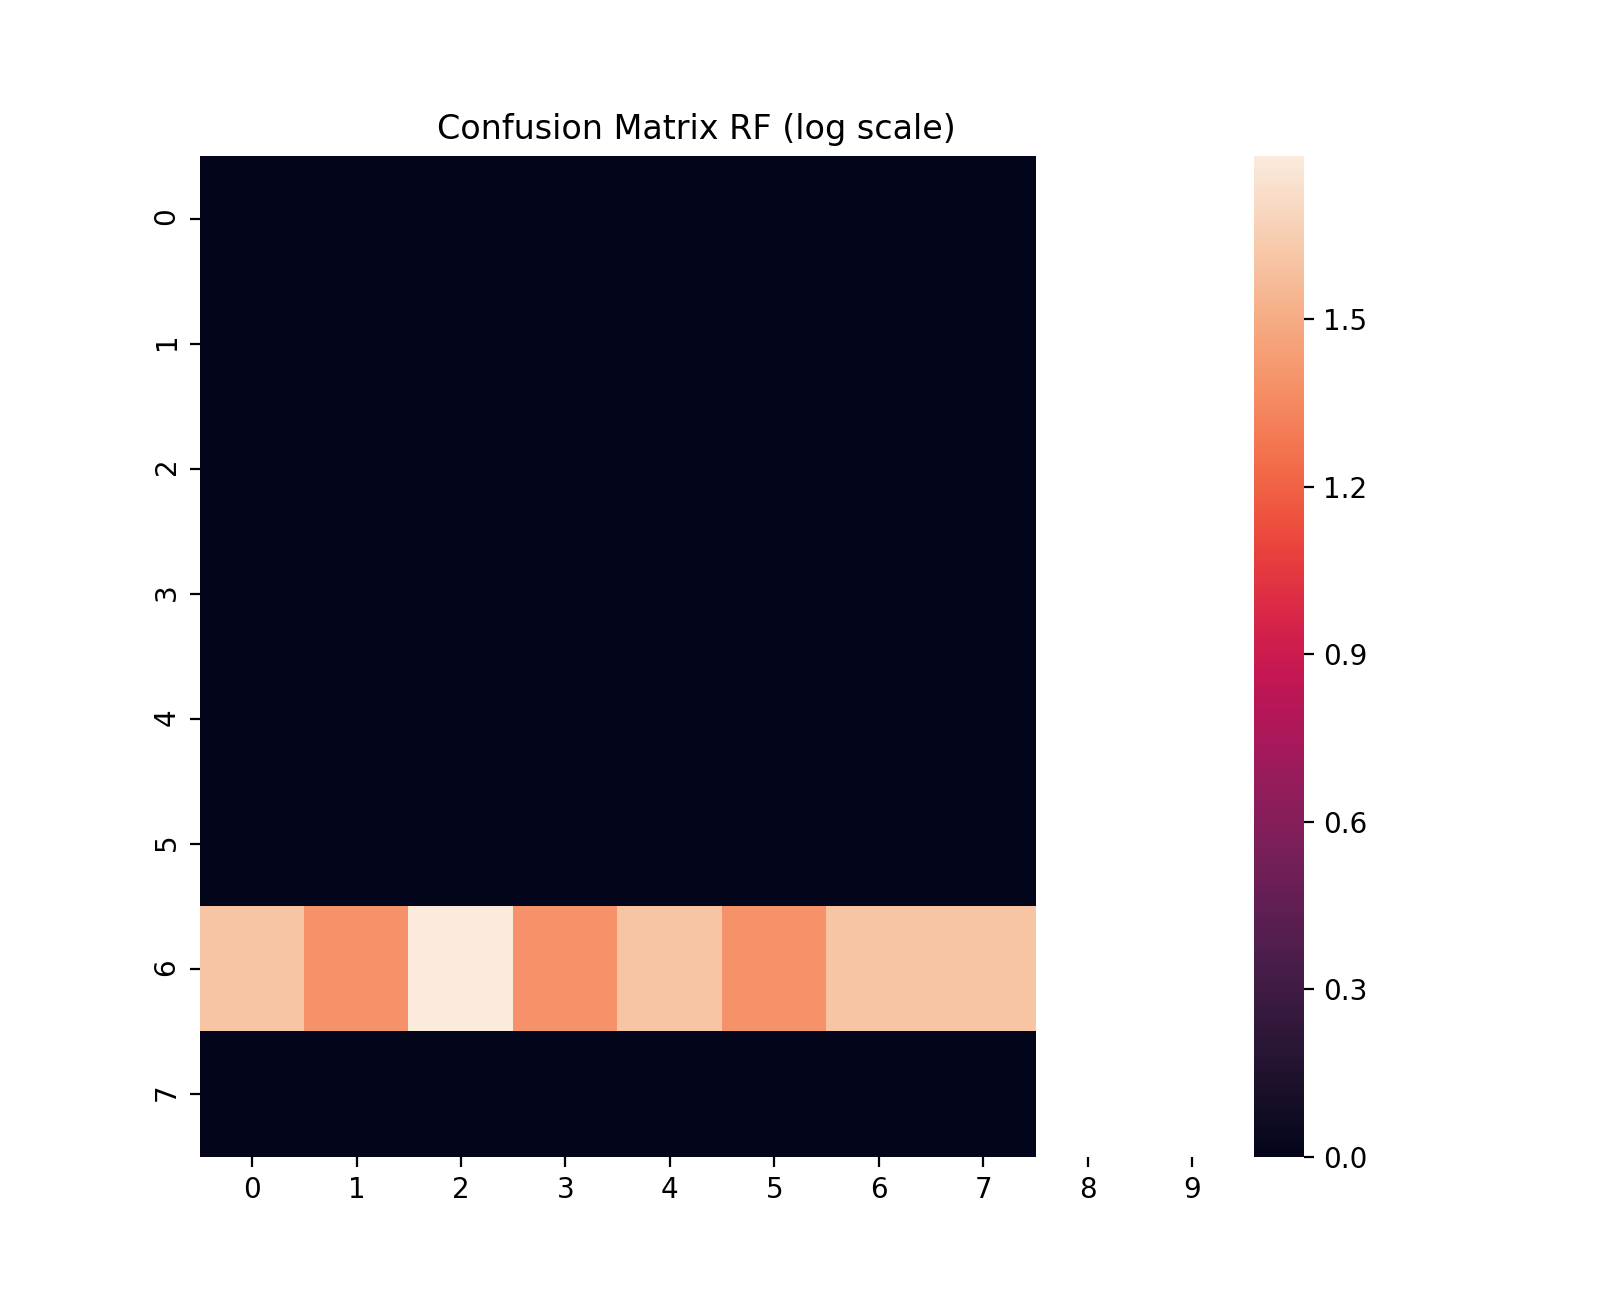
\includegraphics[width=0.8\linewidth]{finaltradconf}
\caption{Matriz de confusión para RF}
\label{fig:conf_rf}
\end{figure}

\begin{table}[H]
	\centering
	\begin{tabular}{|c|c|c|}
		\toprule
		Modelo & Valor de pérdida & Precisión\\
		\hline	
		LR & 0.045492 & 38.21\% \\
		KNN & 0.036158 & 24.1\%\\
		RF & 0.03594 & 73.48\%\\
		SGD & 0.062634 & 35.08\%\\
		SVM & 0.048544 & 28.39\%\\

		\bottomrule
	\end{tabular}
	\caption{Tabla de resultados para CNN}
	\label{tab:res_trad}
\end{table}


\subsection{Redes neuronales convolucionales}


En la figura \ref{fig:cnn1}, correspondiente a la prueba con el modelo pre-entrenado, es posible ver que el valor de pérdida desde el inicio no es alto y disminuye gradualmente con cada época del entrenamiento hasta llegar a un valor muy cercano a 0. Observando la gráfica de la evolución de la precisión, es notoria la diferencia entre el desempeño con las imágenes de entrenamiento (azul) y el desempeño entre las imágenes de validación (naranja). Asimismo, en la figura \ref{fig:cnn2}, correspondiente al rendimiento del modelo en modo de entrenamiento, es posible ver que la precisión con el conjunto de entrenamiento es muy cercana al 100\% y la precisión en la validación queda por debajo, alrededor de 85\%. Esto nos indica que está existiendo un sobreajuste hacia el conjunto de entrenamiento.

\begin{table}[H]
	\centering
	\begin{tabular}{|c|c|c|}
		\toprule
		Conjunto & Valor de pérdida & Precisión\\
		\hline	
		Validación &  0.40 & 88.02\% \\
		Prueba & 2.02 & 36.67\%\\
		\bottomrule
	\end{tabular}
	\caption{Tabla de resultados para CNN}
	\label{tab:res_cnn}
\end{table}

En la matriz de confusión para los resultados del modelo (figura \ref{fig:conf_cnn}) es posible ver la distribución de los resultados predichos. Es posible apreciar que existen dos clases que nunca aparecieron en las predicciones. Las clases con mayor cantidad de aciertos fueron la 5 y la 7 (mientras más claro el color, mayor frecuencia). Finalmente en la figura \ref{fig:rend} podemos ver de manera gráfica el desempeño del modelo. Como se puede observar los resultados de la prueba están dentro del rango de precisión reportado en la tabla \ref{tab:res_cnn}.

\begin{figure}[H]
	\begin{subfigure}{0.5\textwidth}
		\centering
		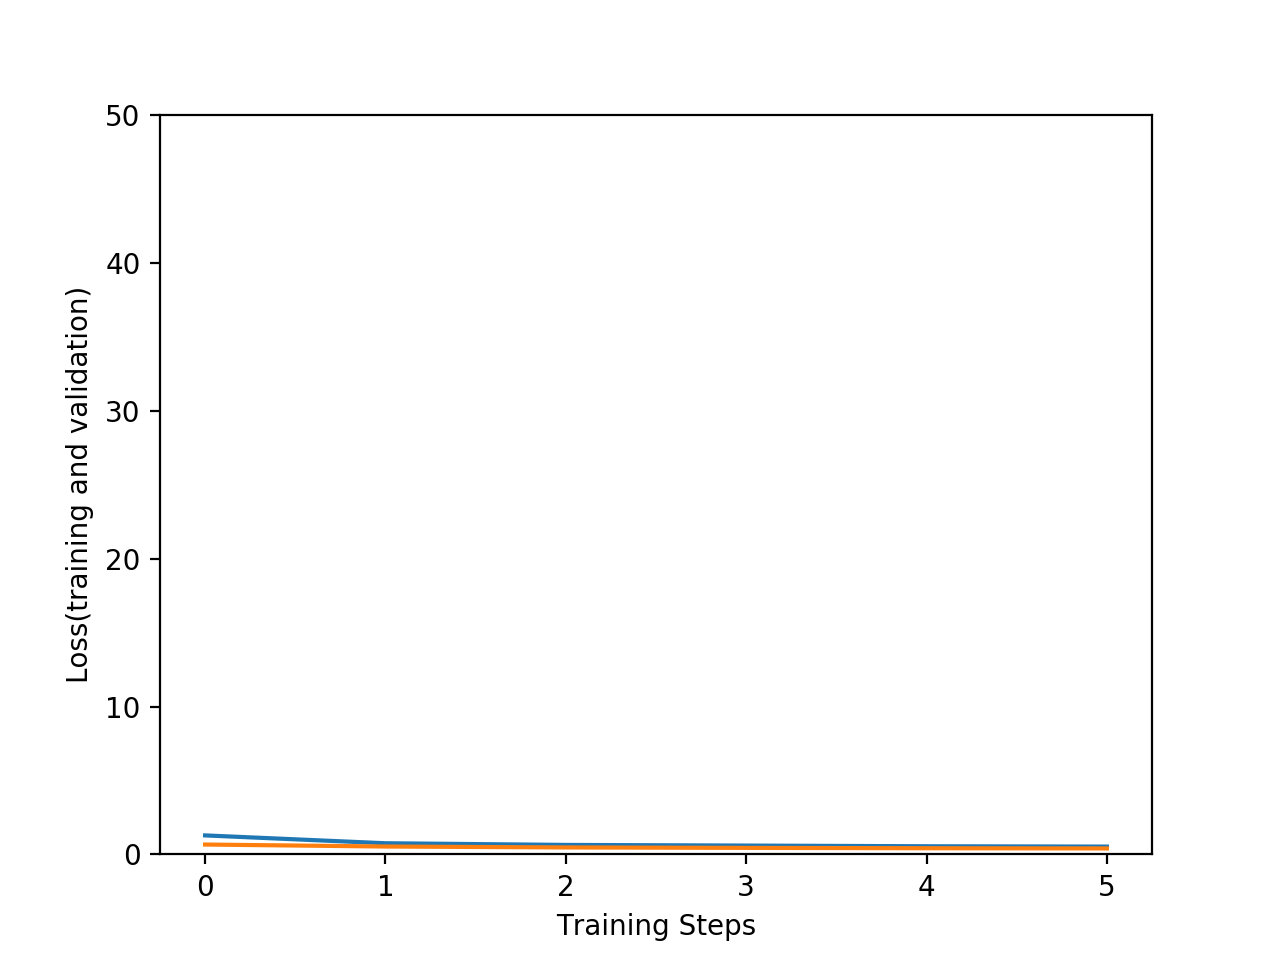
\includegraphics[width=0.8\linewidth]{loss2000}
		\caption{Valor de pérdida}
	\end{subfigure}
	\begin{subfigure}{0.5\textwidth}
		\centering
		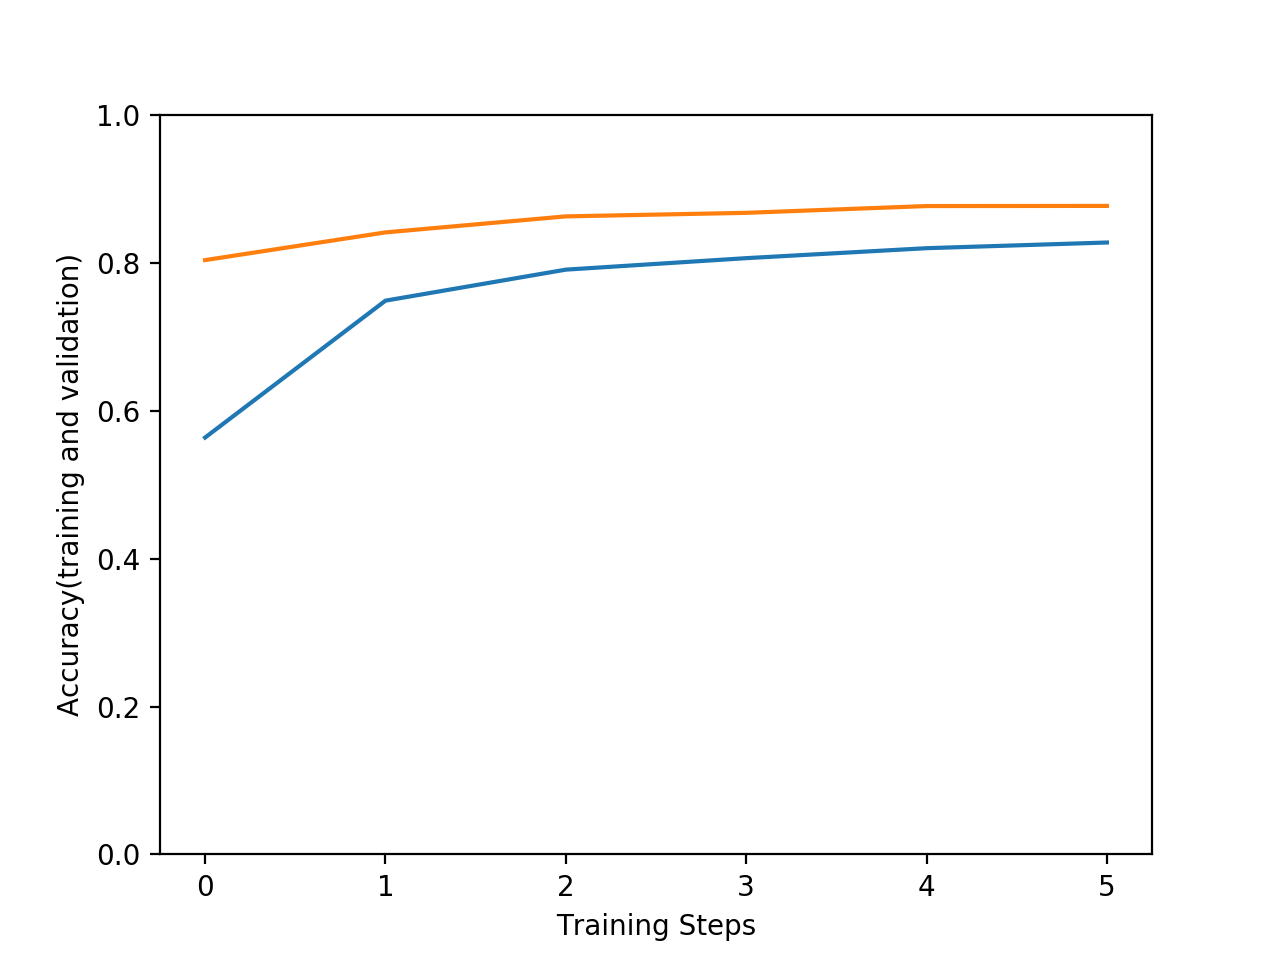
\includegraphics[width=0.8\linewidth]{acc2000}
		\caption{Precisión de entrenamiento}
	\end{subfigure}
	\caption{Desempeño con 2000 datos de modelo pre-entrenado}
	\label{fig:cnn1}
\end{figure}


\begin{figure}[H]
	\begin{subfigure}{0.5\textwidth}
		\centering
		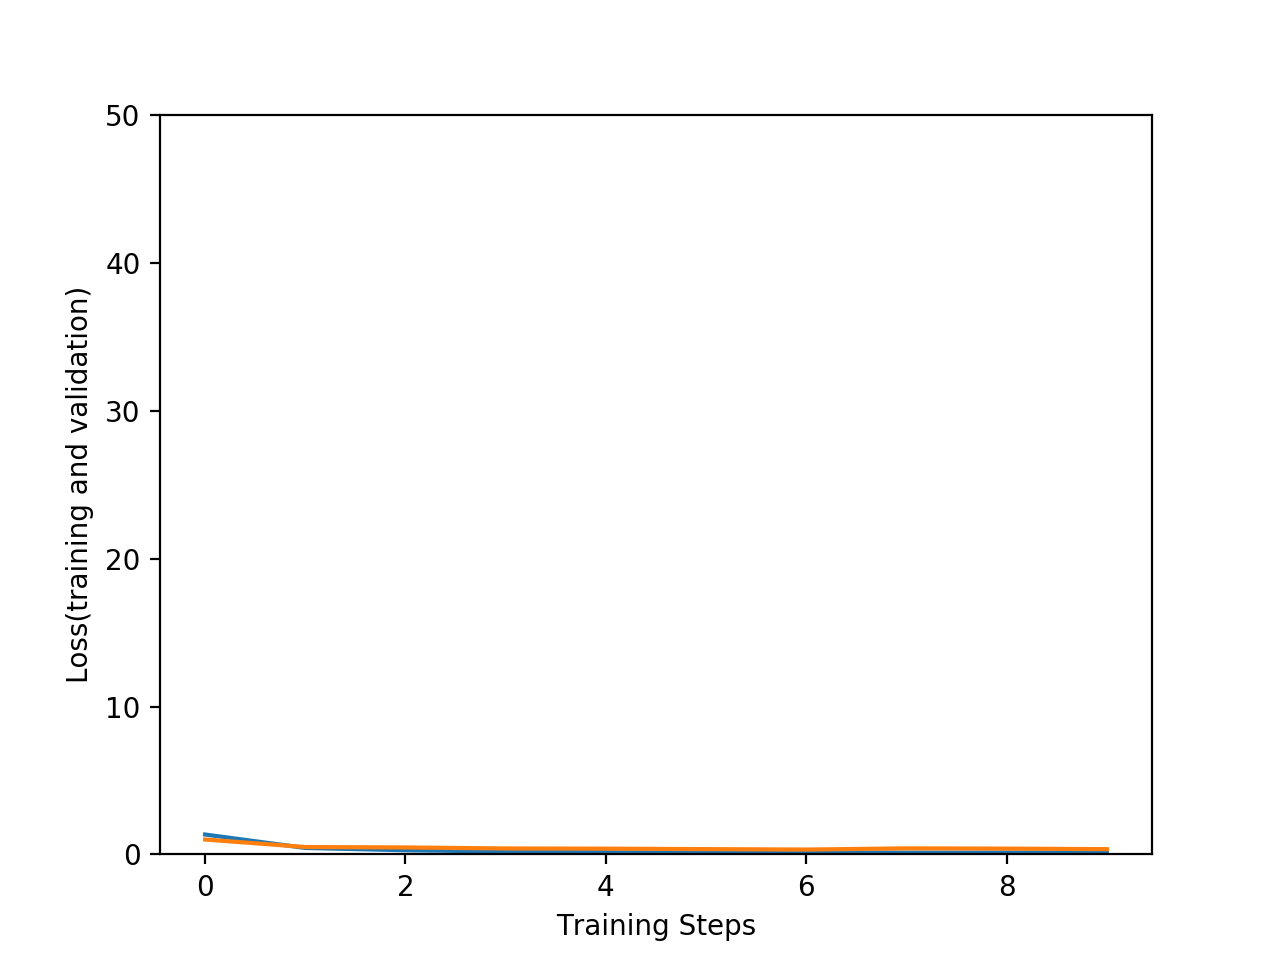
\includegraphics[width=0.8\linewidth]{losstm2}
		\caption{Valor de pérdida}
	\end{subfigure}
	\begin{subfigure}{0.5\textwidth}
		\centering
		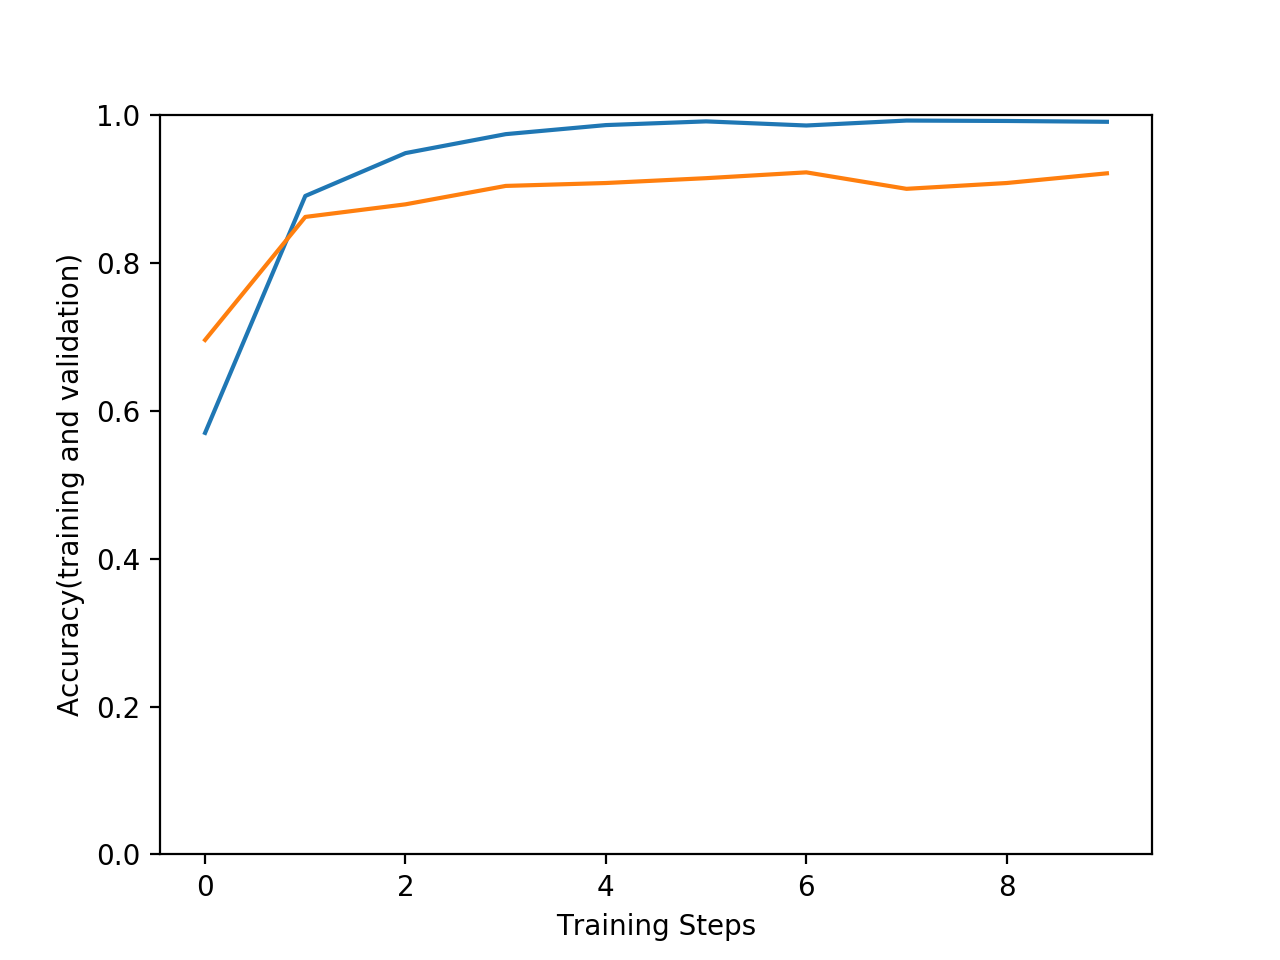
\includegraphics[width=0.8\linewidth]{acctm2}
		\caption{Precisión de entrenamiento}
	\end{subfigure}
	\caption{Desempeño con 2000 datos de modelo en modo entrenamiento}
	\label{fig:cnn2}
\end{figure}


\begin{figure}
	\begin{subfigure}{0.5\textwidth}
		\centering
		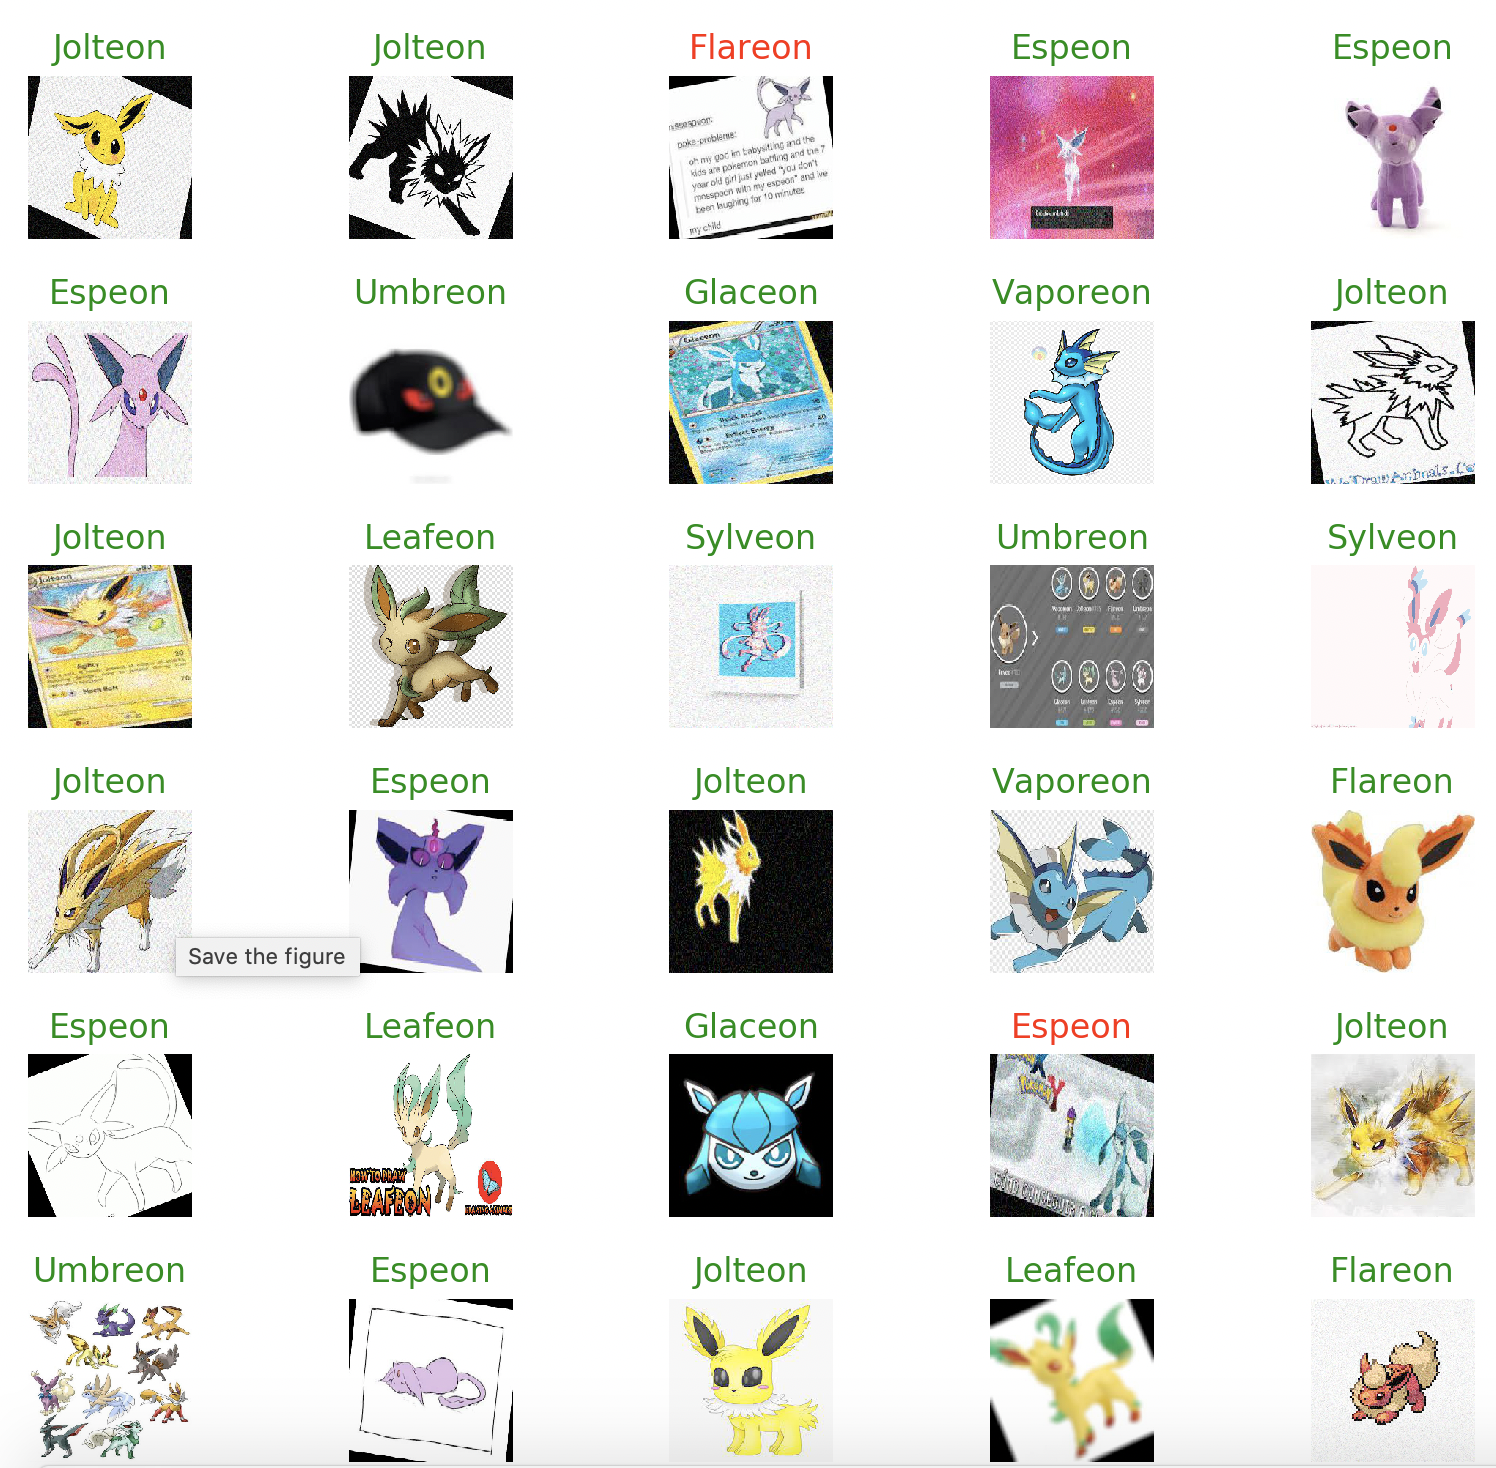
\includegraphics[width=0.8\linewidth]{finalcnnacc}
		\caption{Resultados de validación}
	\end{subfigure}
	\begin{subfigure}{0.5\textwidth}
		\centering
		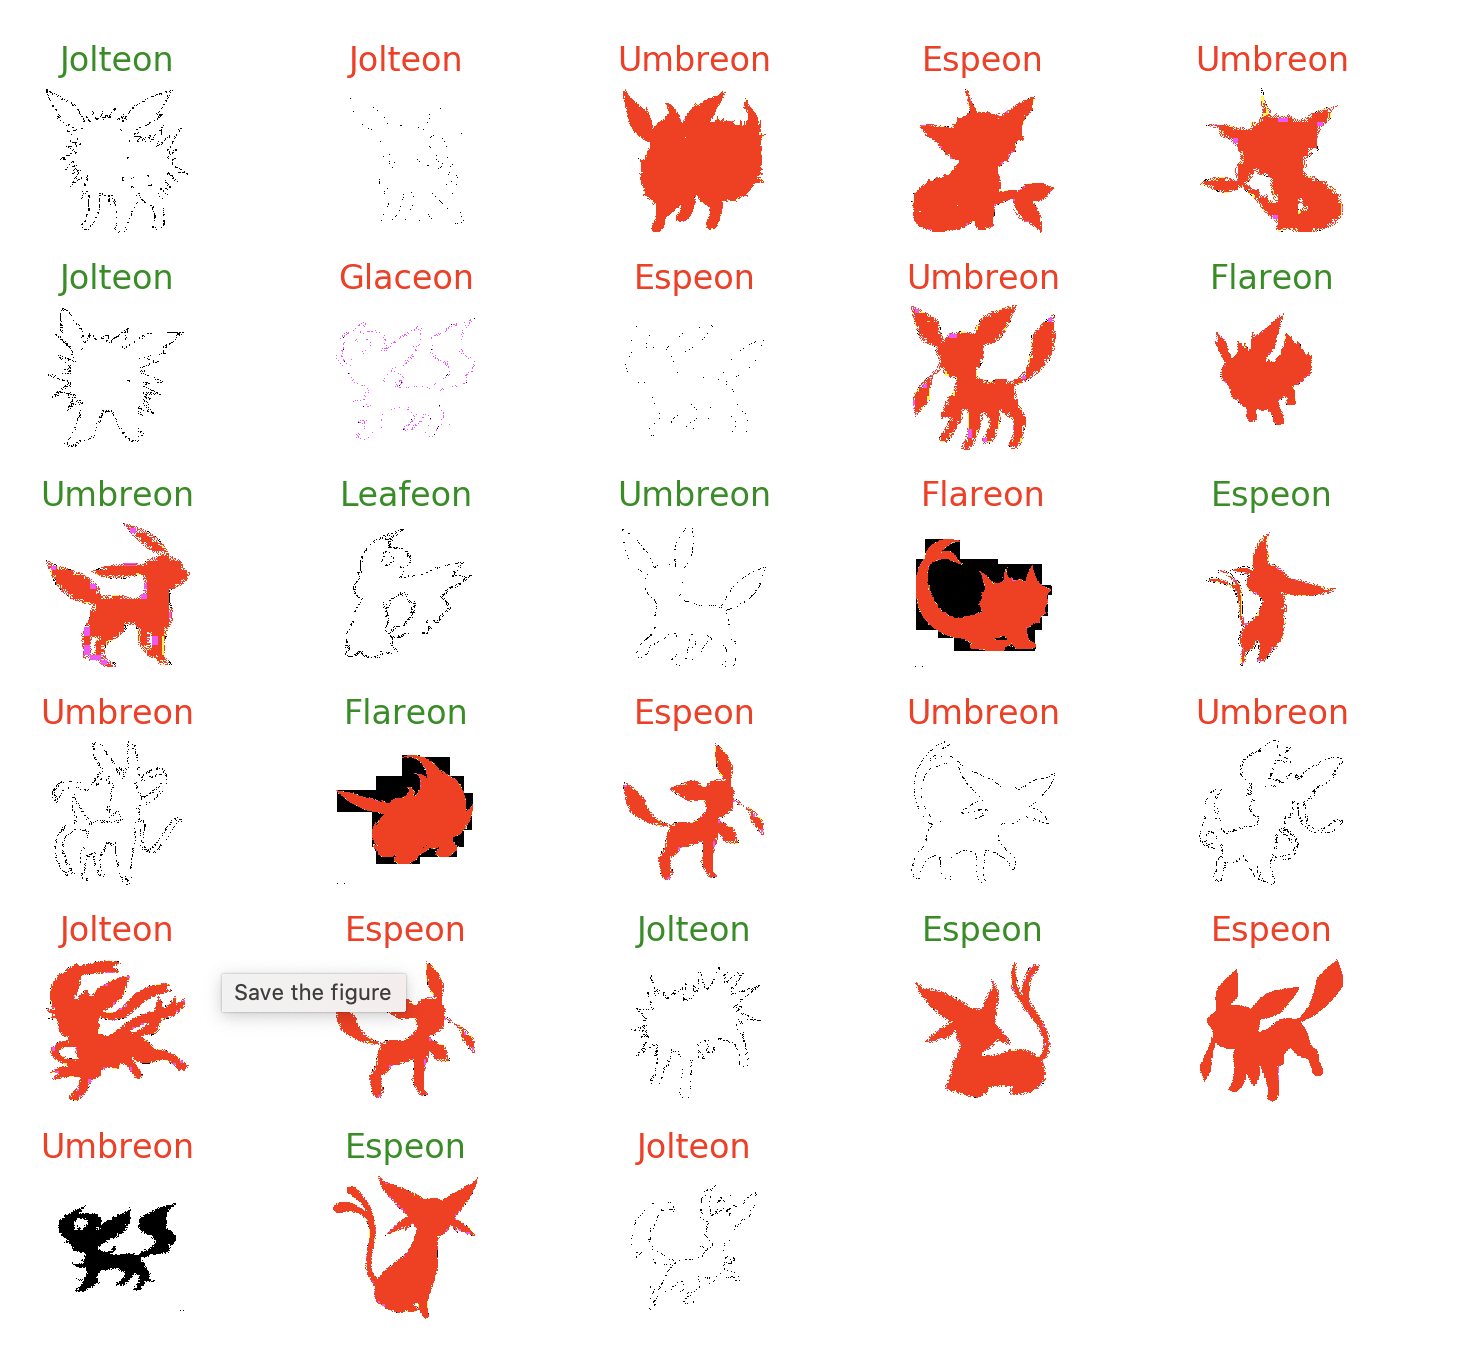
\includegraphics[width=0.8\linewidth]{finalcnnpred}
		\caption{Resultados de predicción}
	\end{subfigure}
	\caption{Comparación de rendimiento}
	\label{fig:rend}
\end{figure}


\begin{figure}[H]
	\centering
	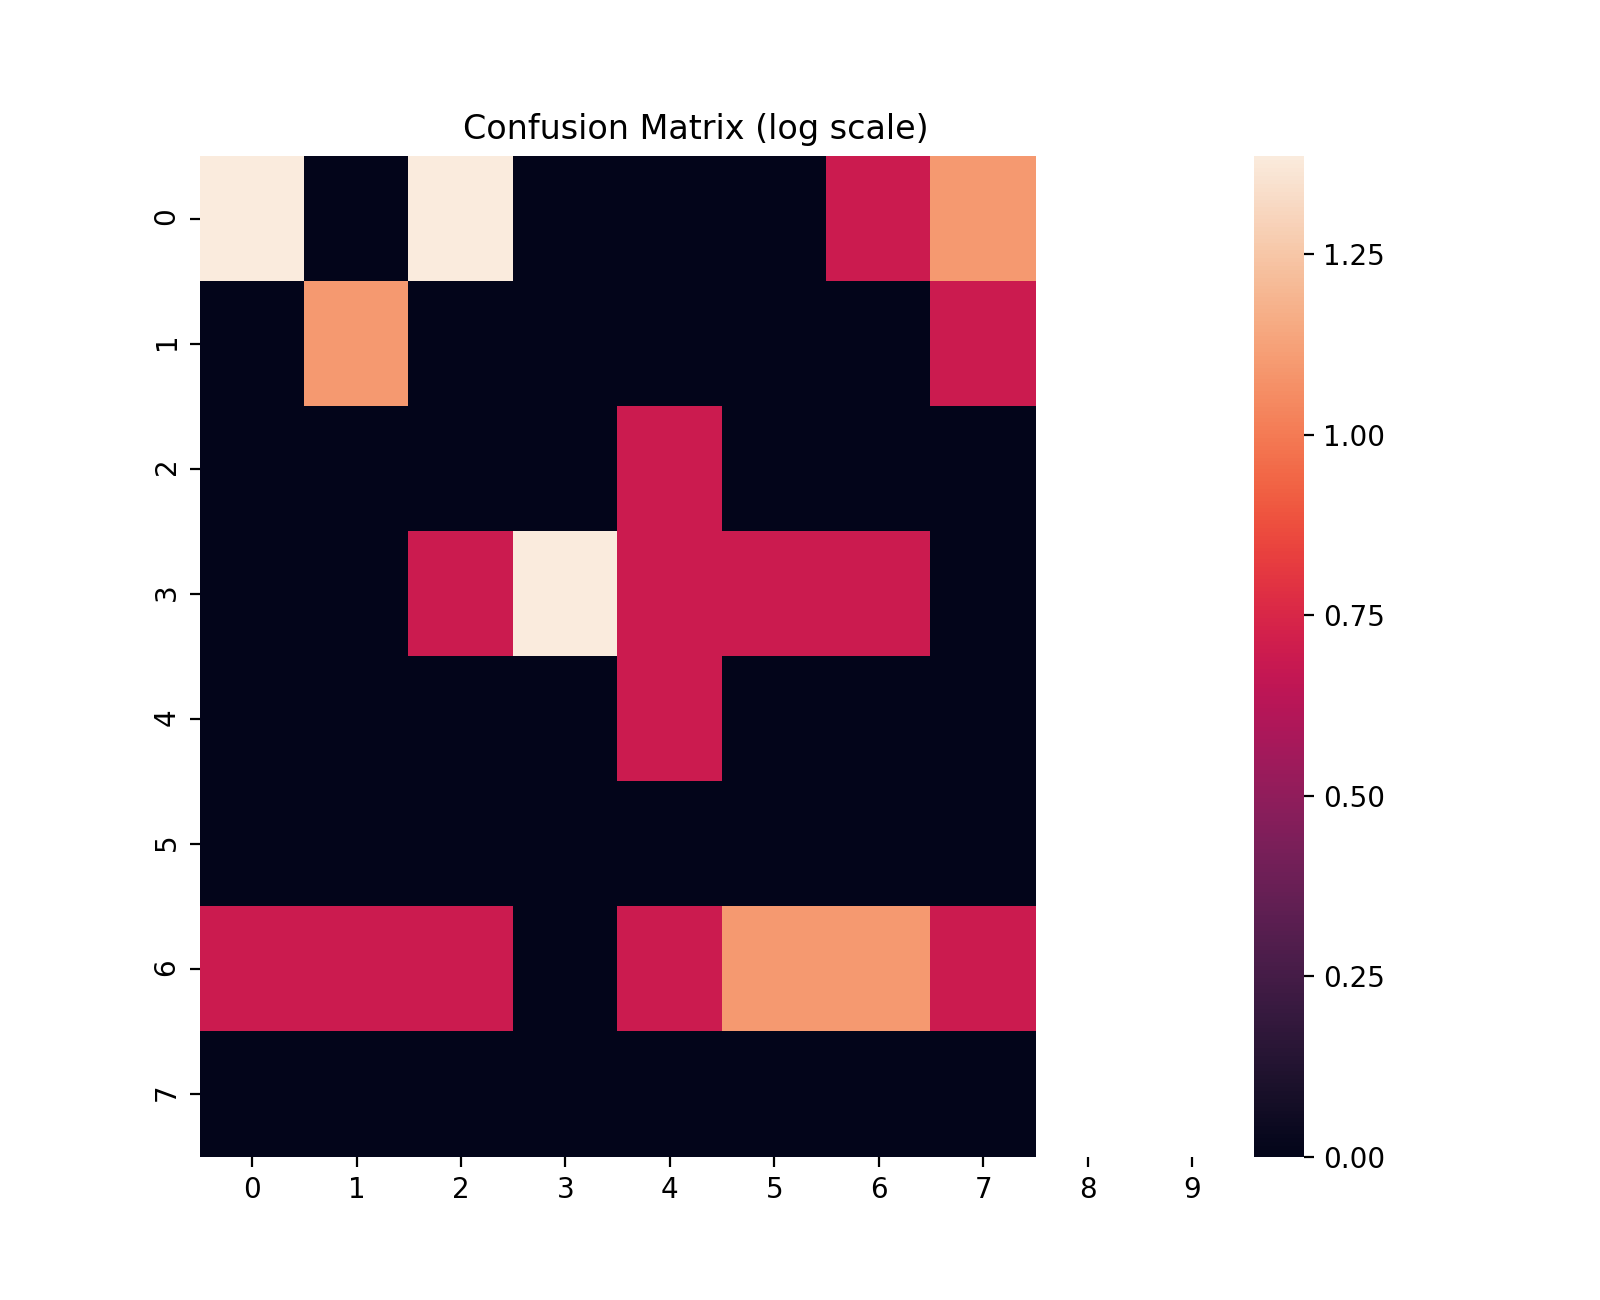
\includegraphics[width=0.8\linewidth]{finalmat}
	\caption{Matriz de confusión para CNN}
	\label{fig:conf_cnn}
\end{figure}

\section{Conclusiones}

La diferencia de desempeño entre el modelo de CNN y los clasificadores tradicionales es clara. Es posible que la extracción de características de manera manual sea la causa de la falla en los modelos tradicionales, pues las imágenes de prueba al no tener características de color o texturas, este tipo de método de extracción podría no ser ideal.  En el caso del modelo de CNN vemos que logra tener un desempeño aceptable.  Sin embargo, es recomendable explorar maneras de alcanzar un mejor desempeño, como utilizar técnicas de aprendizaje por transferencia. La calidad del conjunto de datos podría ser un aspecto a considerar en el desempeño del modelo CNN y los métodos tradicionales; si bien se utilizó un proceso de incremento de datos para lograr tener un conjunto de tamaño significativo, tener un conjunto considerable de imágenes diferentes podría tener un efecto positivo en el desempeño de los modelos. En el caso del modelo de CNN una manera de buscar una mejora en el desempeño sería probar con diferentes modelos de optimización, además de las mejoras en el conjunto de datos ya descritas. 

\bibliography{refereces}
\bibliographystyle{plain}
\end{document}
